\documentclass[12pt]{article}

% a template that a friend gave, it's worked well enough for me
% i have added some packages and stuff that have proved useful

\usepackage{fancyhdr}
\usepackage{tipa}
\usepackage{fontspec}
\usepackage{amsfonts}
\usepackage{enumitem}
\usepackage[margin=1in]{geometry}
\usepackage{graphicx}
\usepackage{float}
\usepackage{amsmath}
\usepackage{braket}
\usepackage{amssymb}
\usepackage{booktabs}
\usepackage{hyperref}
\usepackage{mathtools}
\usepackage{xcolor}
\usepackage{float}
\usepackage{algpseudocodex}
\usepackage{titlesec}
\usepackage{bbm}

\pagestyle{fancy}
\fancyhf{} % sets both header and footer to nothing
\lhead{Kevin Sheng}
\setmainfont{Comic Neue}
\renewcommand{\headrulewidth}{1pt}
\setlength{\headheight}{0.75in}
\setlength{\oddsidemargin}{0in}
\setlength{\evensidemargin}{0in}
\setlength{\voffset}{-.5in}
\setlength{\headsep}{10pt}
\setlength{\textwidth}{6.5in}
\setlength{\headwidth}{6.5in}
\setlength{\textheight}{8in}
\renewcommand{\headrulewidth}{0.5pt}
\renewcommand{\footrulewidth}{0.3pt}
\setlength{\textwidth}{6.5in}
\usepackage{setspace}
\usepackage{multicol}
\usepackage{float}
\setlength{\columnsep}{1cm}
\setlength\parindent{24pt}
\usepackage [english]{babel}
\usepackage [autostyle, english = american]{csquotes}
\MakeOuterQuote{"}

\setlength{\parskip}{6pt}
\setlength{\parindent}{0pt}

\titlespacing\section{0pt}{12pt plus 4pt minus 2pt}{0pt plus 2pt minus 2pt}
\titlespacing\subsection{0pt}{12pt plus 4pt minus 2pt}{0pt plus 2pt minus 2pt}
\titlespacing\subsubsection{0pt}{12pt plus 4pt minus 2pt}{0pt plus 2pt minus 2pt}

\hypersetup{colorlinks=true, urlcolor=blue}

\newcommand{\correction}[1]{\textcolor{red}{#1}}

\usepackage{fancyvrb}

\rhead{Math 168}

\DeclareMathOperator{\Fr}{Fr}
\DeclareMathOperator{\Tr}{Tr}
\newcommand{\lra}{\xLeftrightarrow}
\newcommand{\ra}{\xRightarrow}

\setlist[enumerate,1]{label=(\alph*)}

\begin{document}

\section{Newman 10.2}\label{sec:p1}

\begin{enumerate}
      \item Since $p$ is a probability distribution, all its outputs must sum to one:
            \[\sum_{k=0}^{\infty} Ca^k=1\]
            Assuming $a < 1$ so that the series converges, we have
            \[\sum_{k=0}^{\infty} Ca^k=\frac{C}{1-a}=1 \implies \boxed{C=1-a}\]

      \item We start our summation at $k$ instead of $0$:
            \[P=\sum_{l=k}^{Ca^l} (1-a)a^l =\boxed{a^k}\]

      \item Nodes of degree $w \ge k$ contribute $w$ to the number of ends of edges, so
            \[W = \frac{\sum_{i=k}^{\infty} i(1-a)a^i}{\sum_{i=0}^{\infty} i(1-a)a^i}\]
            Both these summations are the same, just with different starts.
            Let's evaluate the numerator:
            \begin{align*}
                  \sum_{i=k}^{\infty} i(1-a)a^i
                   & = k\sum_{i=k}^{\infty} (1-a)a^i + \sum_{i=k}^{\infty} (i-k)(1-a)a^i                  \\
                   & = k\sum_{i=k}^{\infty} (1-a)a^i + \sum_{i=k+1}^{\infty} \sum_{j=i}^{\infty} (1-a)a^j \\
                   & = ka^k + \sum_{i=k+1}^{\infty} a^i                                                   \\
                   & = ka^k + \frac{a^{k+1}}{1-a}
            \end{align*}
            The denominator is just this expression when $k=0$, or $\frac{a}{1-a}$.
            Putting it under the numerator gives
            \begin{align*}
                  P
                   & = \frac{ka^k + \frac{a^{k+1}}{1-a}}{\frac{a}{1-a}} \\
                   & = \frac{ka^k(1-a)+a^{k+1}}{a}                      \\
                   & = \boxed{ka^{k-1}(1-a)+a^k}
            \end{align*}
\end{enumerate}

\section{Newman 10.4}

\begin{enumerate}
      \item Given that the axes use a log-scale, I think the second graph
            with a linear trend is the one that's scale-free.

      \item This is a very rough approximation, but I took log base 10s
            of some lattice-ish points and got $(1, -1.1)$ $(2, -2.2)$ as some sample points.
            Thus, the slope of the graph is $-1.1$ and $\boxed{\alpha \approx 2.1}$.
            We add $1$ since the graph is of the CDF, not the degree distribution itself.

      \item From the textbook we know that for a degree distribution
            that follows the power law, we have
            \[W=P^{(\alpha-2)/(\alpha-1)}\]
            where $W$ is the fraction of edge ends attached
            to the fraction $P$ of highest-degree notes.
            Solving for $W=\frac{1}{2}$ and $\alpha=2.1$ gives around \boxed{0.00049}.
\end{enumerate}

\section{Newman 11.4}

\begin{enumerate}
      \item If we solve $S=1-\exp(-\braket{k}S)$ for $\braket{k}$ when $S=\frac{1}{2}$,
            we have $\boxed{\braket{k}=-2\ln \frac{1}{2} \approx 1.386}$.

      \item Using the approximation from class and our previous approximation of $\braket{k}$, we have
            \[p(5) \approx \frac{\braket{k}^5}{5!}\exp(-\braket{k}) \approx \boxed{0.0107}\]

      \item Of the $n-1$ other nodes, around half are in the component and half aren't.
            The chance that all five of a certain node's neighbors are in the disconnected half
            is about $\frac{1}{2^5}$, since $n$ is large
            and each neighbor has a fifty-fifty chance of being in the giant component.
            Thus, the chance that the node belongs to the giant component
            is $1-\frac{1}{2^5}=\boxed{\frac{31}{32}}$.

      \item We multiply the previous two probabilities
            and double it to get that around \boxed{2.06\%} of the nodes in the giant
            component have degree exactly $5$.
\end{enumerate}

\pagebreak

\section{Random Triangles}

\begin{enumerate}
      \item I'm not sure if this is a trick question, but it seems to be \boxed{1}.
            Every other node is guaranteed to be connected to $v_1$.

      \item We have
            \begin{align*}
                  E[k_i]
                   & = E\left[\sum_{j=1}^{n} \mathbf{1}[(v_j, v_i) \in E]\right] \\
                   & = \sum_{j=1}^{n} P[(v_j, v_i) \in E]                        \\
                   & = \boxed{\sum_{j=1}^{i-1} \frac{1}{j} + \frac{n-i}{i}}
            \end{align*}

      \item Since edges are chosen independently,
            \[P[\text{triangle}] = P[(v_i, v_j) \in E]P[(v_j, v_k) \in E]P[(v_i, v_k) \in E] = \boxed{\frac{1}{i^2j}}\]

      \item We have by PIE
            \[P[\text{at least $2$ edges}]=\frac{1}{i^2}+\frac{1}{ij}+\frac{1}{ij}-\frac{2}{i^2j}=\boxed{\frac{j+2i-2}{i^2j}}\]

      \item The expected values are as follows:
            \begin{gather*}
                  \mathbb{E}[\text{\# triangles}]
                  =\sum_{i < j < k} \frac{1}{ij^2}
                  =\sum_{i=1}^{n} \sum_{j=i+1}^{n} \frac{n-j}{ij^2} \\
                  \mathbb{E}[\text{\# conn. triples}]
                  =\sum_{i < j < k} 3 \cdot \frac{1}{ij^2} + \frac{j+2i-2}{i^2j}
                  = \sum_{i=1}^{n} \sum_{j=i+1}^{n} \frac{(n-j)(j+2i+1)}{i^2j}
            \end{gather*}
            so our expected global clustering coefficient is this monstrosity:
            \[EC=\frac{3 \cdot \sum_{i=1}^{n} \sum_{j=i+1}^{n} \frac{n-j}{ij^2}}
                  {\sum_{i=1}^{n} \sum_{j=i+1}^{n} \frac{(n-j)(j+2i+1)}{i^2j}}\]
\end{enumerate}

\pagebreak

\section{Erdos-Reyni Simulations}

\subsection{Part A}

These are the plots I got:
\begin{center}
      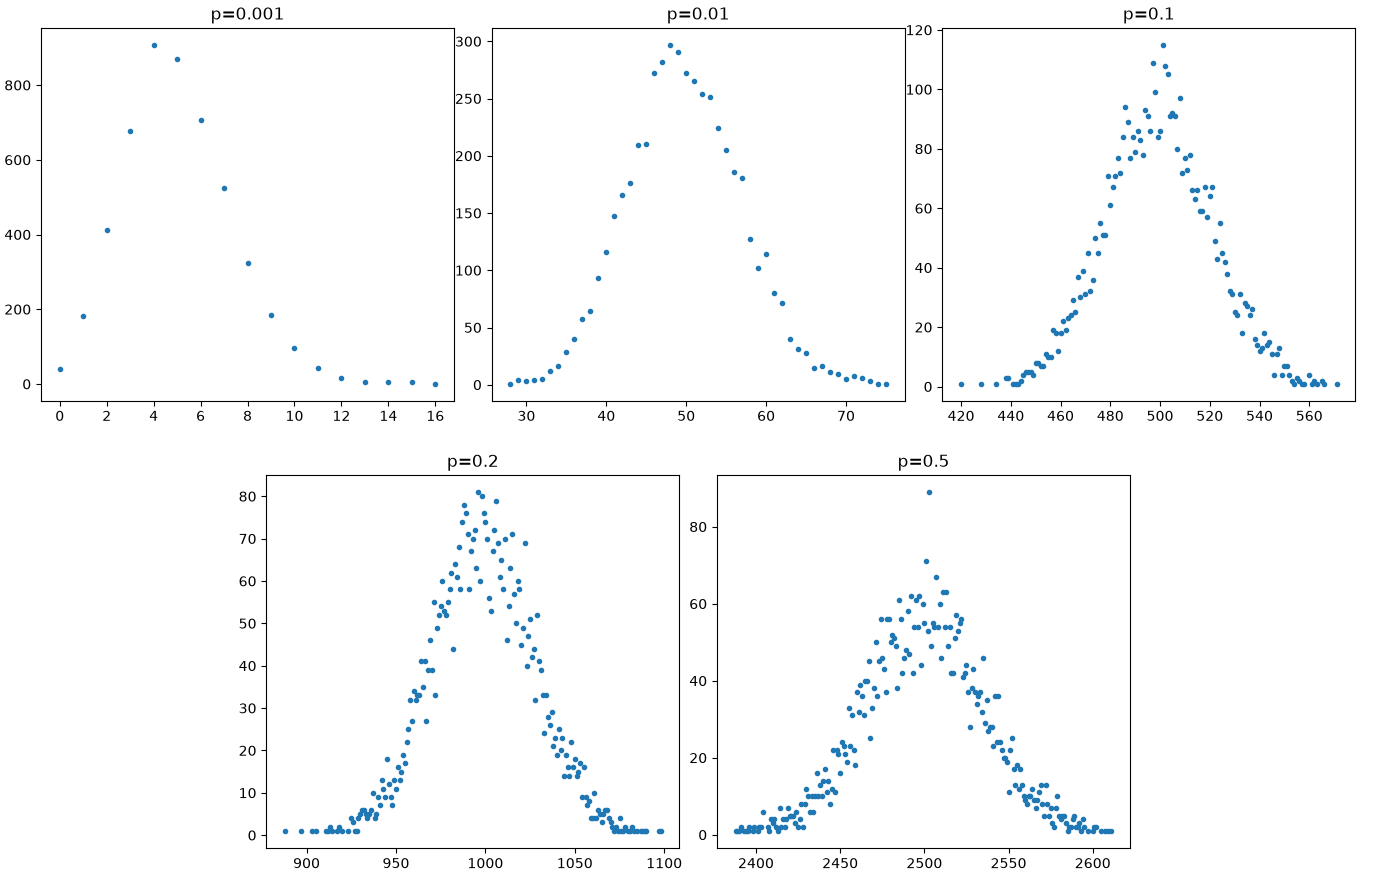
\includegraphics[width=15cm]{img/hw6/degrees}
\end{center}

\subsection{Part B}

All the randomly generated graphs were fully connected except for the
first one where $p=0.001$.
In that graph, the largest connected component had $4966$ nodes.

\pagebreak

\subsection{Part C}

This is the resulting graph:
\begin{center}
      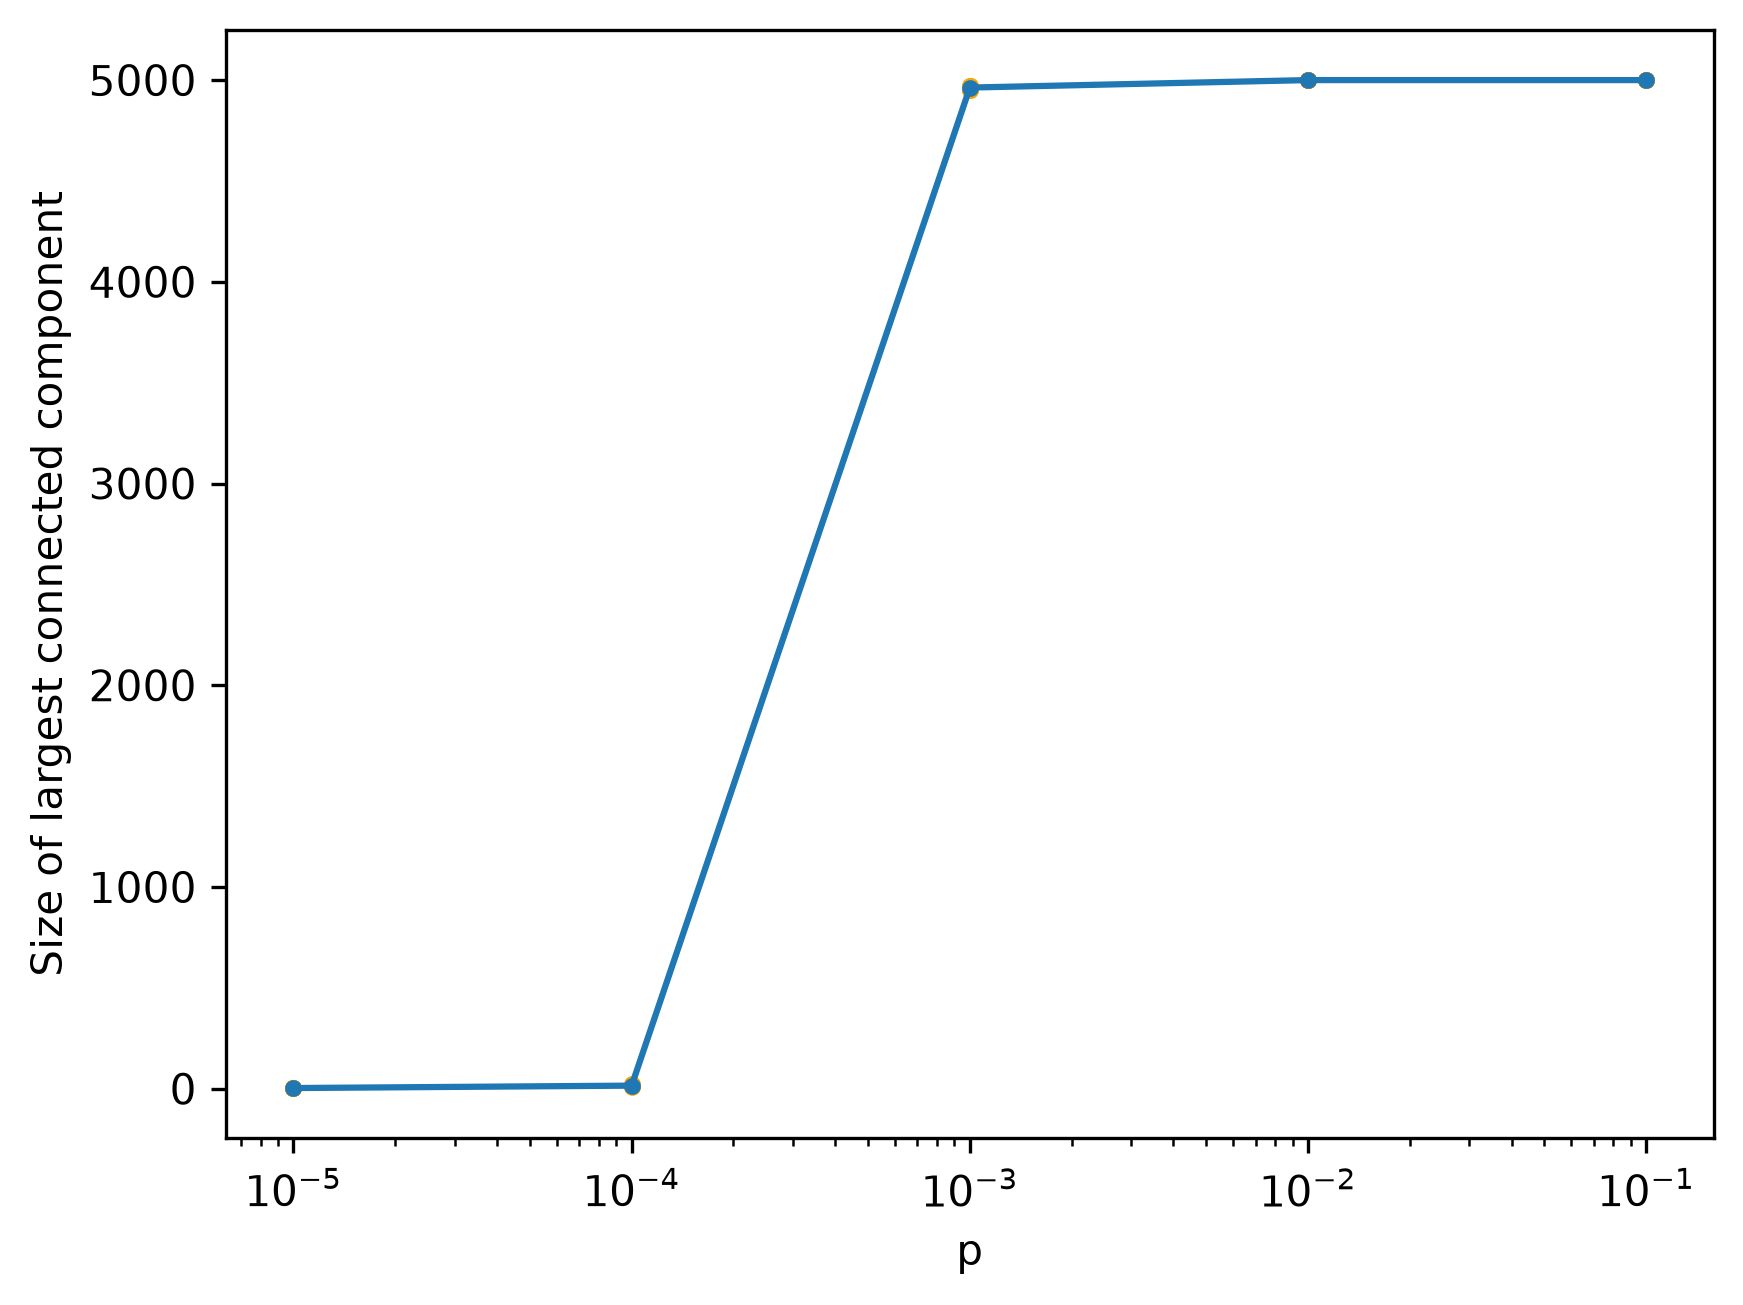
\includegraphics[width=15cm]{img/hw6/cc_sizes}
\end{center}
The blue line connects the means of all the $p$ values, but it doesn't
really matter anyways because at this scale there's basically
no variance in the size of the largest connected component.

\end{document}
